%%≈
\subsection{Jets Mis-identified as Photons}
\label{sec:fakerate}
%%%%%%%%%%%%%%%%%%%%%%%%%%%%%%%%%%%%%%%%%%%%%%%%%%%%%%%%%%%%%%%%%%%%%%%%%%%%%%%%%%%%%%%%%%%%%%%%%%%%%%%%%%%%%%%%%%%%%%%%%%%%%%%%%%%%%%%%%%%%%%%%%%%%%%%%%%%%%%%%%%%%%%
Any analysis involving photons in their final state is sensitive to background coming from jets misidentified as photons.
One of our dominant background sources arises from QCD, typically dijet and multijet events which produce a fake photon.
In particular these fake photons appear when high \met jets fragment mainly into isolated neutral pions (${\pi}^0$s),
which decay via ${\pi}^0 \rightarrow \gamma \gamma$ and are sufficiently collimated to appear as a single electromagnetic shower in the ECAL.
Such jets can mimic an energetic photon and pass our photon selection criteria.
Although the rate of such fragmentation can be small, the large QCD production cross section results in a significant jet-faking-photon background for this analysis.
In this section we present an estimate of the jet-faking-photon background using data driven techniques.

We would like to compute the ratio that a jet would fake a photon (fake ratio).
To reduce possible bias, this procedure is done in a data control sample orthogonal to our signal data sample.
After the fake ratio is derived we apply it to our signal data to estimate the number of jet-faking-photon events.
Moreover, as this ratio is dependent on the photon \et, 
we perform this study in different \et bins and construct a fake ratio as a function of photon \et. Finally we present and examine all possible systematic sources.

%%%%%%%%%%%%%%%%%%%%%%%%%%%%%%%%%%%%%%%%%%%%%%%%%%%%%%%%%%%%%%%%%%%%%%%%%%%%%%%%%%%%%%%%%%%%%%%%%%%%%%%%%%%%%%%%%%%%%%%%%%%%%%%%%%%%%%%%%%%%%%%%%%%%%%%%%%%%%%%%%%%%%%
\subsubsection{Jet $\rightarrow$ Photon Fake Ratio Measurement strategy}
Our control sample is populated by objects reconstructed as photons using the same data sample that is used in our analysis and matching photon objects to the online photons that triggered the signal path by requiring $\Delta R < 0.3$.
Furthermore we apply all noise filters (as described in Sec.~\ref{sec:data}), require at least one good vertex, and select the leading photon with reconstructed photon energy $\pt > 30 \GeV$, within the barrel region.
The orthogonality of the control data sample to the analysis data sample is secured by selecting the missing transverse energy to be $\met < 40 GeV$. The potential topological differences arising from the above selection are later examined and taken into account as a systematic uncertainty of the method.

%%%%%%%%%%%%%%%%%%%%%%%%%%%%%%%%%%%%%%%%%%%%%%%%%%%%%%%%%%%%%%%%%%%%%%%%%%%%%%%%%%%%%%%%%%%%%%%%%%%%%%%%%%%%%%%%%%%%%%%%%%%%%%%%%%%%%%%%%%%%%%%%%%%%%%%%%%%%%%%%%%%%%%
%\subsubsection{Strategy}
We construct initially what is called the raw fake ratio; 

\begin{equation}FR_{raw}=\frac{numerator}{denominator}\end{equation}

In the above definition, \textbf{numerator} is populated by photon objects passing Medium ID and isolation criteria as recomended by $e-\gamma$ POG. In particular, the ID criteria are:

\begin{itemize}
\item Pixel Seed Veto
\item $R9>0.9$
\item $H/E<0.05$
\item $\sigma_{i\eta i\eta} < 0.011$
\item PF Charged Hadron Isolation $ < 1.5$
\item PF Neutral Hadron Isolation $ < 1.0+0.04\times p_{T}^{\gamma}$
\item PF Photon Isolation $ < 0.7+0.005\times p_{T}^{\gamma}$
\end{itemize}

In addition, we require $\sigma_{i\eta i\eta} > 0.001$ and $\sigma_{i\phi i\phi} > 0.001$, along with the swiss cross cut mentioned earlier in order to reject spikes and beam halo background events. 
A pixel seed veto is applied so that we do not select electrons misidentified as photons.

On the other hand we populate the \textbf{denominator} with jets which could fake photons, constructing a sample orthogonal to numerator, using very loose photon ID and isolation criteria and requiring concurrently at least one of the isolation criteria, or $\sigma_{i\eta i\eta}$, to have failed. 
This leads to the construction of a lower and upper bound on isolation criteria. 
We also require $\sigma_{i\eta i\eta} < 0.015$ to reduce the contamination from beam halo events which characteristically peak at high values of $\sigma_{i\eta i\eta}$. 
More details on this cut can be find in Appendix B. Explicitly our denominator ID criteria are:

\begin{itemize}
\item pixel seed veto
\item $R9>0.9$
\item $H/E<0.05$
\item $\sigma_{i\eta i\eta}<0.015$
\end{itemize}

while the upper bound denominator cuts are:

\begin{itemize}
\item PF Charged Hadron Isolation $ < min\{5\times4.0,0.2\times p_{T}^{\gamma}\}$
\item PF Neutral Hadron Isolation $ < min\{5\times(4.5+0.04\times p_{T}^{\gamma}), 0.2\times p_{T}^{\gamma}\}$
\item PF Photon Isolation $ < min\{5\times(4.5+0.005\times p_{T}^{\gamma}), 0.2\times p_{T}^{\gamma}\}$
\end{itemize}

and the lower bound denominator cuts are:

\begin{itemize}
\item $\sigma_{i\eta i\eta} > 0.012 $ \newline
\textbf{OR}  PF Charged Hadron Isolation $ > 4.0$ \newline
\textbf{OR}  PF Neutral Hadron Isolation $ > 4.5+0.04\times p_{T}^{\gamma}$ \newline
\textbf{OR}  PF Photon Isolation $ > 4.5+0.005\times p_{T}^{\gamma}$
\end{itemize}

Both numerator and denominator have the isolation variables $\rho$ corrected, as recommended by $e-\gamma$ POG.
Fig. \ref{fig:rawFR} shows the raw fake ratio as defined for seven different photon \pt bins.

\begin{figure}[hbtp]
\begin{center}
%\includegraphics[width=0.6\columnwidth]{qcd_plots/rawFR}
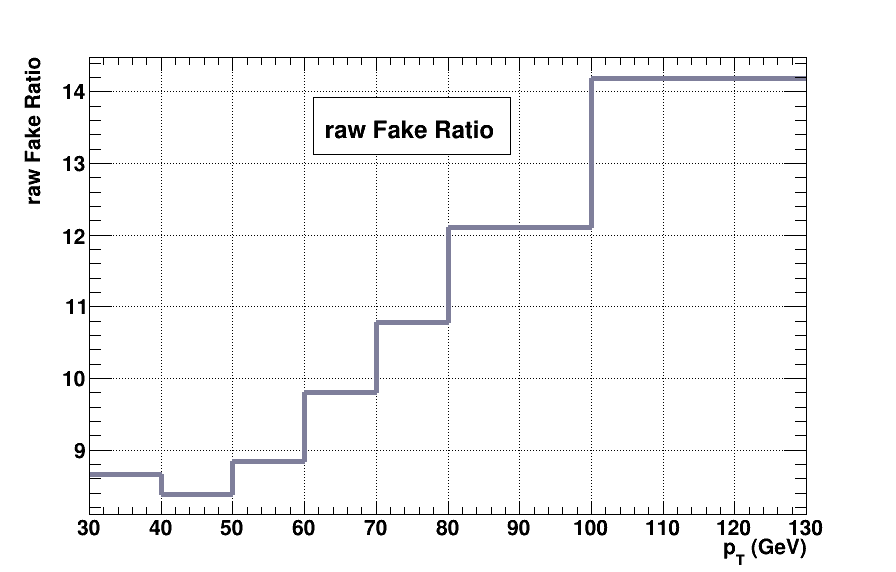
\includegraphics[width=0.6\columnwidth]{qcdPlots/qcd_rawFR.png}
\caption{Raw fake ratio values per photon \et bin.}
\label{fig:rawFR}
\end{center}
\end{figure}

%%%%%%%%%%%%%%%%%%%%%%%%%%%%%%%%%%%%%%%%%%%%%%%%%%%%%%%%%%%%%%%%%%%%%%%%%%%%%%%%%%%%%%%%%%%%%%%%%%%%%%%%%%%%%%%%%%%%%%%%%%%%%%%%%%%%%%%%%%%%%%%%%%%%%%%%%%%%%%%%%%%%%%
\subsubsection{Subtracting true photon contamination}

The numerator sample will be contaminated by a considerable fraction of true isolated photons from inclusive QCD direct photon production. This contribution needs to be estimated and subtracted to identify the true QCD fake ratio. We subtract these true photons using the template method. Due to this subtraction, the corrected fake ratio, then becomes:

\begin{equation}
FR_{corrected}=\frac{numerator-contamination}{denominator}
\end{equation}

The cleaning of the numerator of real photons is done through the template method. We use $\sigma_{i\eta i\eta}$ templates to distinguish between real and fake photons in the numerator sample. We construct our fake photon template by applying numerator like cuts to our data control sample (withtout the $\sigma_{i\eta i\eta}$ cut) in a sideband region of charged hadron isolation :

\begin{itemize}
\item $2.0 GeV <$ PF Charged Hadron isolation$<6.0 GeV$
\end{itemize}

The extraction of the templates for real photon shapes is done using Monte Carlo samples. In particular we have used $\gamma +$ Jets MC, applying numerator cuts again 
without the $\sigma_{i\eta i\eta}$ requirement and taking the leading reconstructed photon object that is also matched in $\Delta R$ to a generated photon. 

%We have analyzed the following samples:

%\begin{itemize}
%\item {/G\_Pt-*to*\_TuneZ2star\_8TeV\_pythia6/Summer12\_DR53X-PU\_S10\_START53\_V7A-v1}
%\end{itemize} 

A $\sigma_{i\eta i\eta}$ correction prescription is applied to real templates in order to match data \cite{higgs2GammaAN}. 
In particular we rescale $\sigma_{i\eta i\eta}$ to 

\begin{equation}
\sigma_{i\eta i\eta}^{scaled} = 0.891832 \times \sigma_{i\eta i\eta} + 0.0009133
\label{eqn:fr}
\end{equation}

as recommended by the $H \rightarrow \gamma \gamma$ group. We construct the real (MC-gen matched), 
fake (data-sideband) and data (data-numerator) $\sigma_{i\eta i\eta}$ templates for seven different photon \et bins of:

\begin{equation}
 [30-40], [40-50], [50-60], [60-70], [70-80], [80-100], [100-130] \GeV
\end{equation}

A likelihood fit using ROOFIT is then performed, of $real + fake$ templates to $data$ templates per $\ET^{\gamma}$.
Fig. \ref{fig:medTemplates1} and \ref{fig:medTemplates2} show the templates per photon \et bin after performing the fit.

\begin{figure}[hbtp]
\begin{center} 
$\begin{array}{cc}
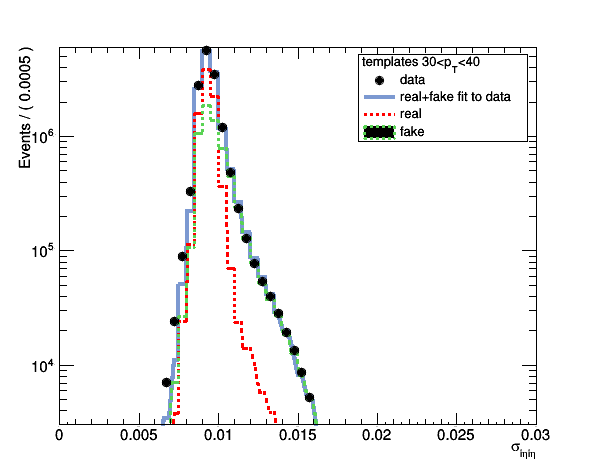
\includegraphics[width=0.4\columnwidth]{qcdPlots/qcd_template_1} &
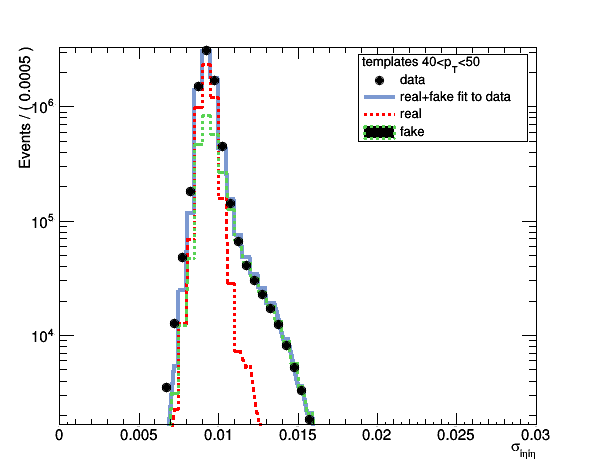
\includegraphics[width=0.4\columnwidth]{qcdPlots/qcd_template_2} \\
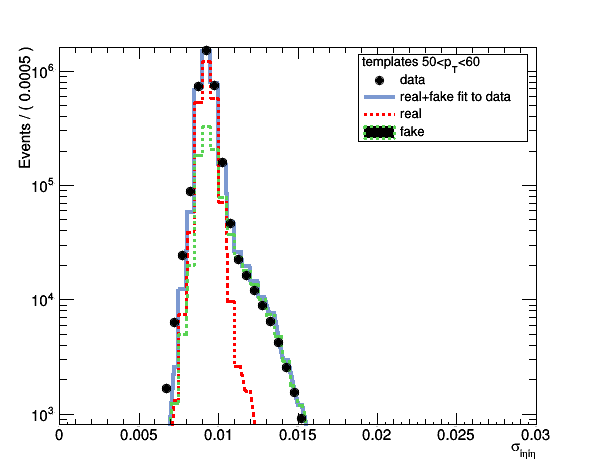
\includegraphics[width=0.4\columnwidth]{qcdPlots/qcd_template_3} &
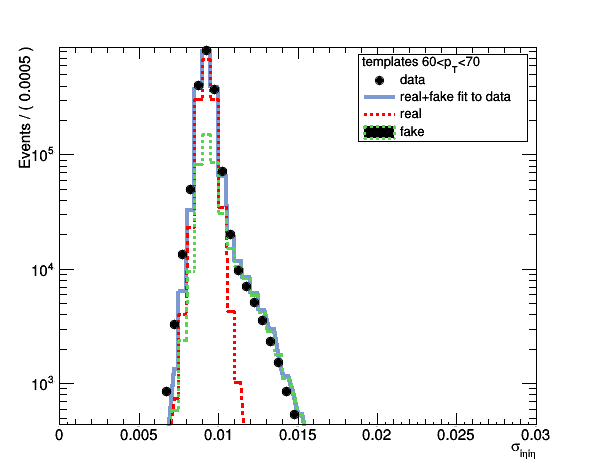
\includegraphics[width=0.4\columnwidth]{qcdPlots/qcd_template_4}
\end{array} $
\caption{$\sigma_{i\eta i\eta}$ templates for different photon \et bin.}
\label{fig:medTemplates1}
\end{center}
\end{figure}
%%-------------------------------------------------------------------------------
\begin{figure}[hbtp]
\begin{center} 
$\begin{array}{cc}
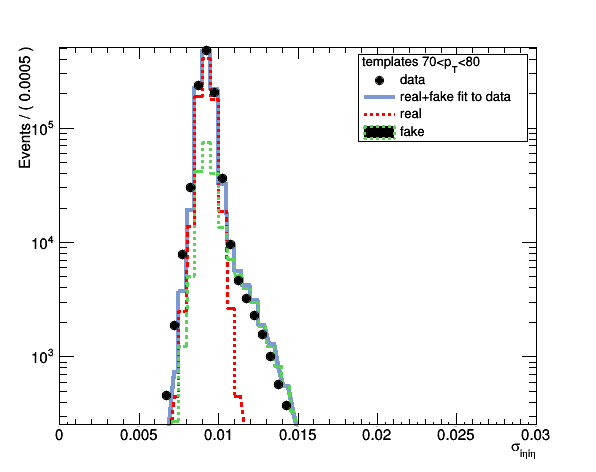
\includegraphics[width=0.4\columnwidth]{qcdPlots/qcd_template_5} &
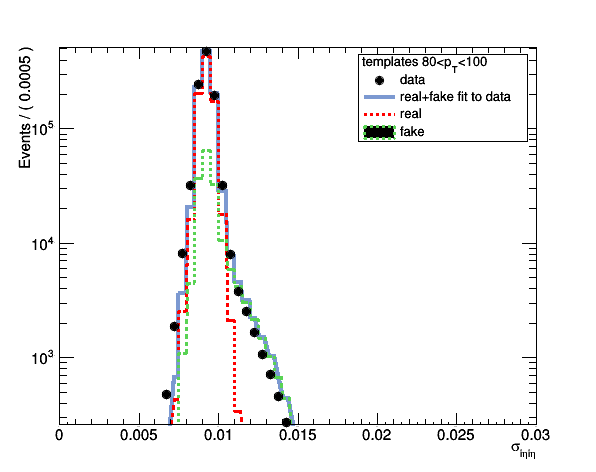
\includegraphics[width=0.4\columnwidth]{qcdPlots/qcd_template_6} \\
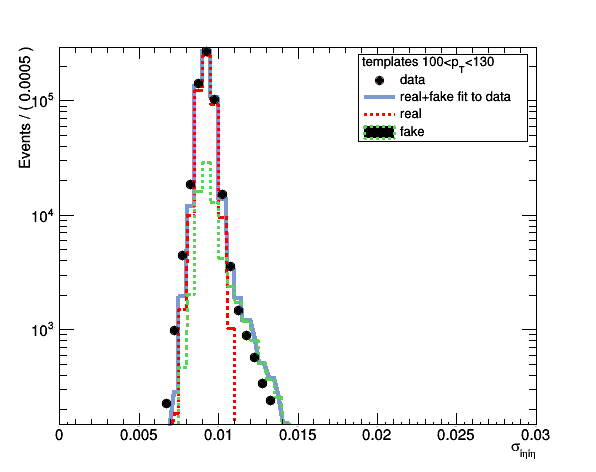
\includegraphics[width=0.4\columnwidth]{qcdPlots/qcd_template_7} &
\end{array} $
\caption{$\sigma_{i\eta i\eta}$ templates for different photon \et bin.}
\label{fig:medTemplates2}
\end{center}
\end{figure}

The yields of the real photons in the region of $\sigma_{i\eta i\eta}<0.011$ is called the contamination and is subtracted from the numerator yields, following equation~\ref{eqn:fr}.

%%%%%%%%%%%%%%%%%%%%%%%%%%%%%%%%%%%%%%%%%%%%%%%%%%%%%%%%%%%%%%%%%%%%%%%%%%%%%%%%%%%%%%%%%%%%%%%%%%%%%%%%%%%%%%%%%%%%%%%%%%%%%%%%%%%%%%%%%%%%%%%%%%%%%%%%%%%%%%%%%%%%%%
\subsubsection{Estimation of jet $\rightarrow$ photon mismeasurement ratio} 
As we have found the contamination in numerator, the corrected fake ratio is then calculated per photon \et bin, by simply subtracting the real photon contribution from raw numerator. We then perform a final fit for the seven FR bins and obtain the final corrected fake ratio as a function of \et.
The function we have used to parametrize the FR is;

\begin{equation}
f_{\ET^{\gamma}} = p0 + \frac{p1}{(\ET^{\gamma})^{p2}}
\end{equation}

Fig. \ref{fig:fitResult} shows the corrected fake ratio as a function of photon \et. It should be noted that, given our disjoint selection of numerator and denominator samples, these samples are not subset of each other. Therefore, one can expect a ratio $>$ 1.

\begin{figure}[hbtp]
\begin{center}
%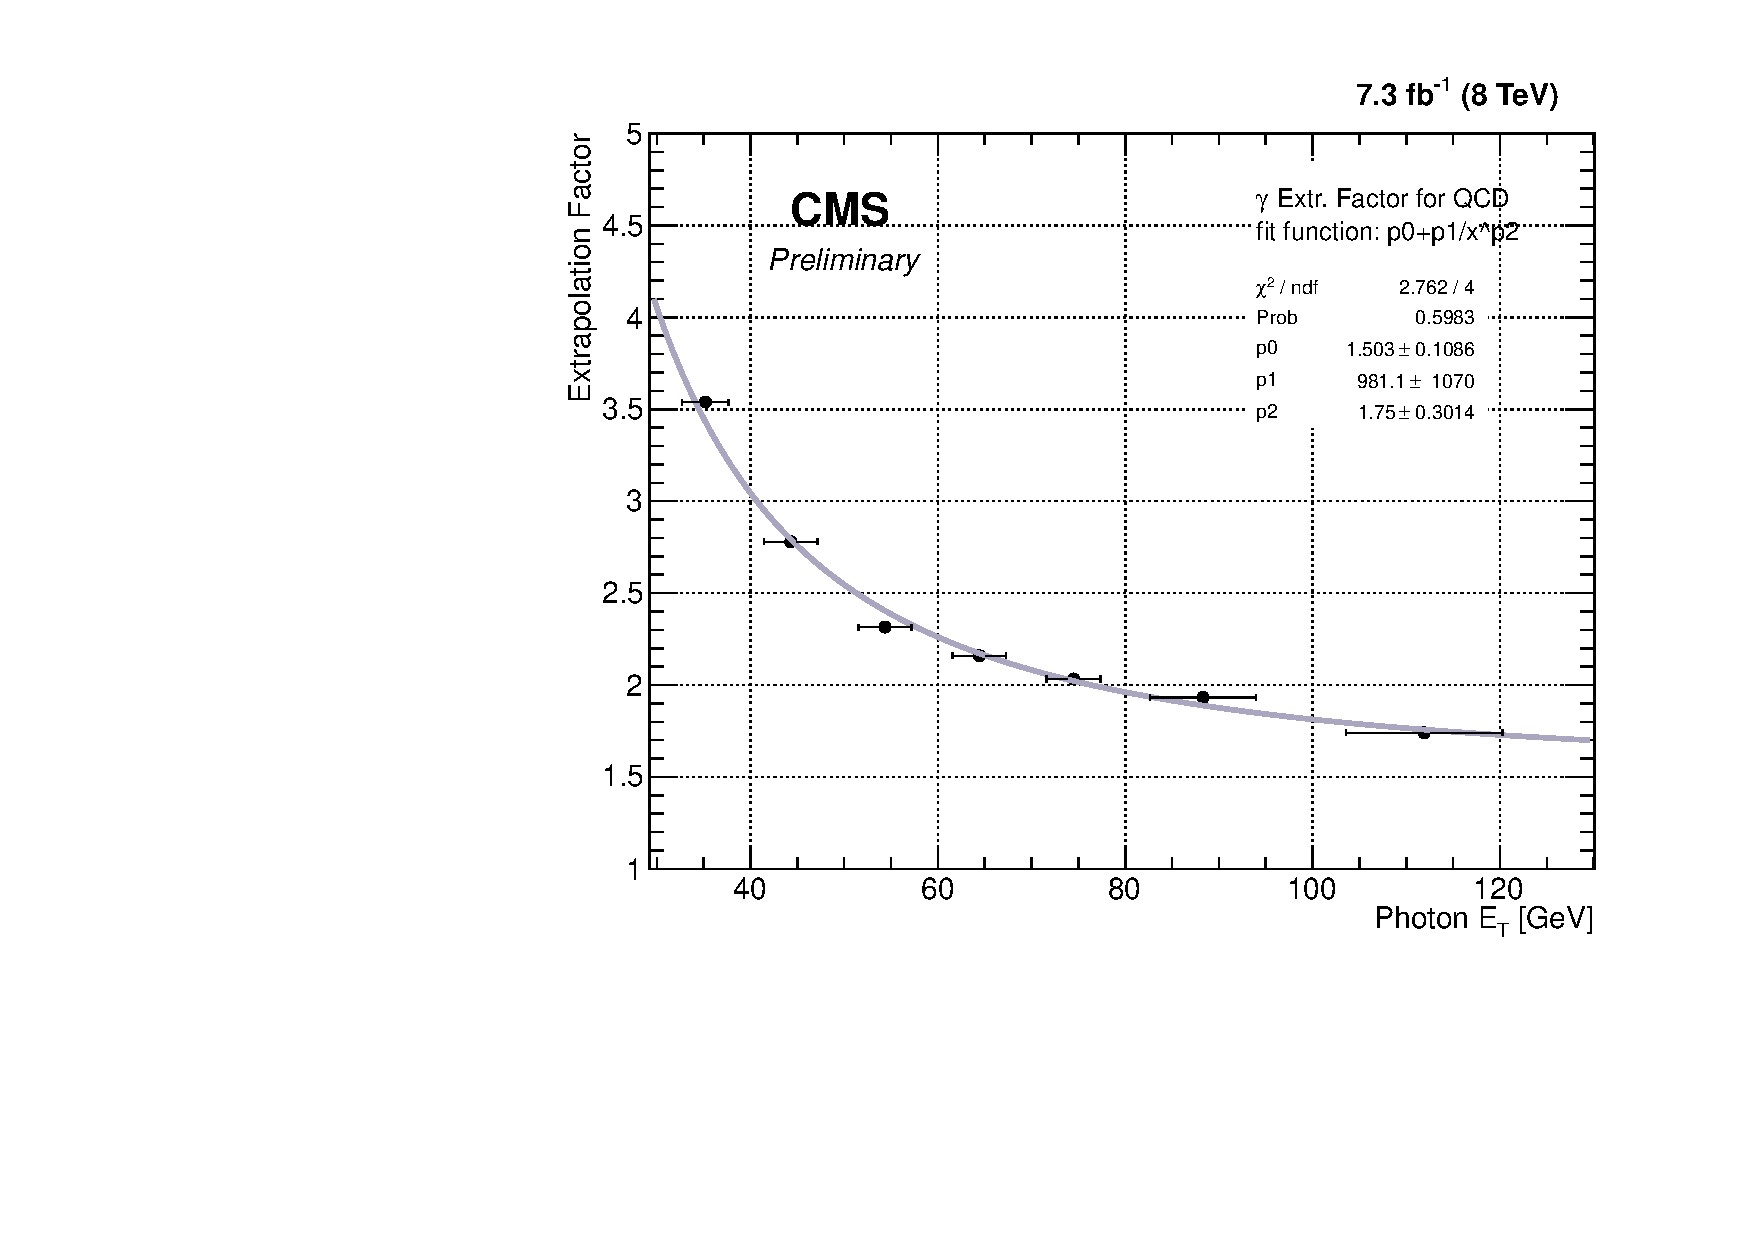
\includegraphics[scale=0.5]{qcd_plots/fitResult.pdf}
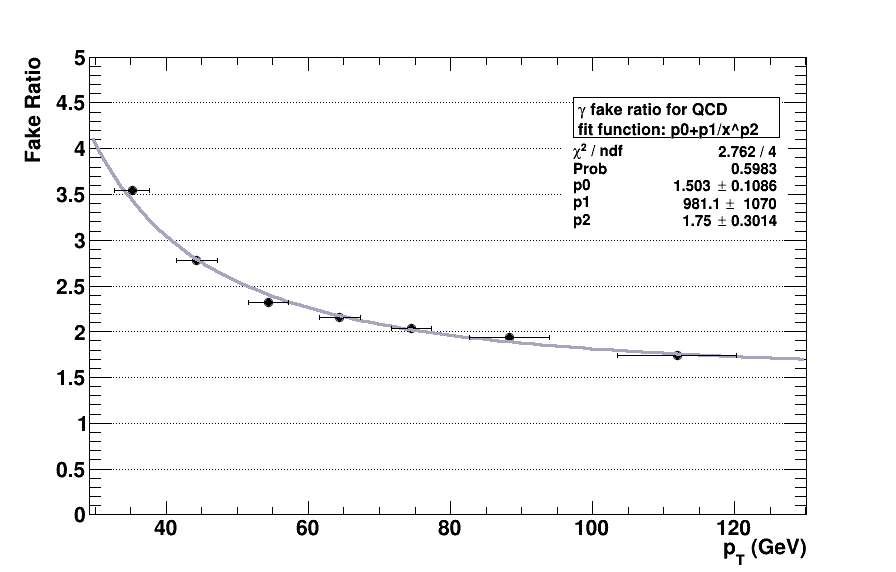
\includegraphics[scale=0.5]{qcdPlots/qcd_fitResult}
\caption{Final corrected fake ratio as a function of photon \et.}
\label{fig:fitResult}
\end{center}
\end{figure}

In this plot, the x-axis points and errors are calculated by looking at the mean and rms of the photon $\pt$ distribution in each $\pt$ bin. 
The errors on the y-axis are calculated through error propogation based on the fit errors. 
Finally, the QCD yield is estimated by applying the above function to the reconstructed photons of our analysis data sample,
which pass our basic selection cuts, but have the photon selection replaced by denominator selection cuts.

%%%%%%%%%%%%%%%%%%%%%%%%%%%%%%%%%%%%%%%%%%%%%%%%%%%%%%%%%%%%%%%%%%%%%%%%%%%%%%%%%%%%%%%%%%%%%%%%%%%%%%%%%%%%%%%%%%%%%%%%%%%%%%%%%%%%%%%%%%%%%%%%%%%%%%%%%%%%%%%%%%%%%%
\subsubsection{Jet $\rightarrow$ photon mismeasurement systematics} 
The main source of systematics on this procedure are estimated by examining the following;

\begin{itemize}
\item $\sigma_{i\eta i\eta}$ template binning
\end{itemize}

Template \textbf{binning} is examined and found to have almost negligible contribution. In particular we have recalculated the fake ratio by creating templates with half and
double bin size to estimate the photon contamination. This change in $\sigma_{i\eta i\eta}$ is found to not affect the final fake ratio estimate as can be seen in Fig. \ref{fig:fit_BINNINGsys}.

\begin{figure}[hbtp]
\begin{center}
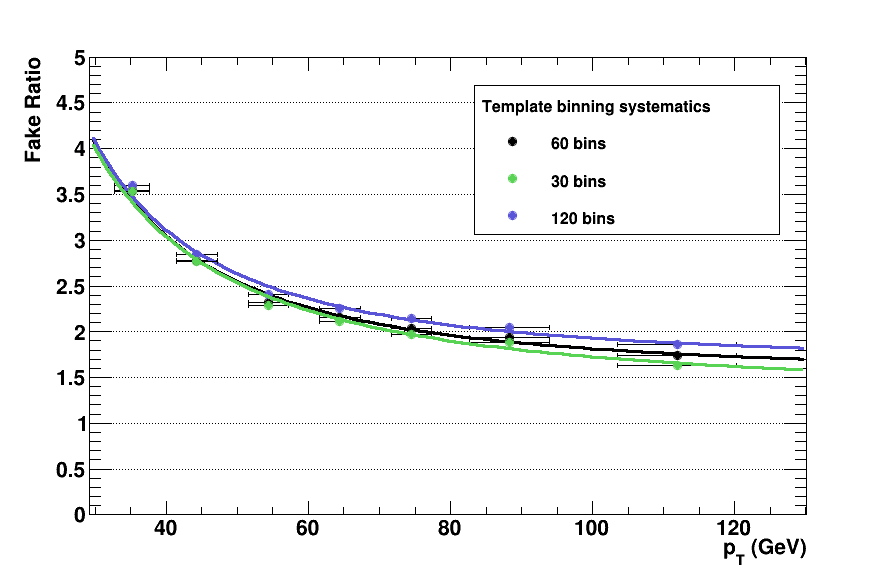
\includegraphics[width=0.7\columnwidth]{qcdPlots/qcd_fitResult_Binning}
\caption{Corrected fake ratio as a function of photon \et for different template binning.}
\label{fig:fit_BINNINGsys}
\end{center}
\end{figure}

\begin{itemize}
\item denominator definition
\end{itemize}

In order to calculate \textbf{denominator} systematics, we have altered the denominator definition by changing the lower bound definition of denominator selection cuts.
We have required one of the "OR" statements of the lower bound not to be present for each case. This has been performed for the PH and NH isolation statements in the lower bound criteria.  The following cuts are applied in both cases in their lower bounds:

\begin{itemize}
\item $ 0.015 > \sigma_{i\eta i\eta} > 0.012 $ \newline
\item\textbf{OR}  PF Charged Hadron Isolation $ > 4.0$ \newline
\item\textbf{OR}  PF Neutral Hadron Isolation $ > 4.5+0.04\times p_{T}^{\gamma}$ \newline
\end{itemize}

The cases differ by:
\begin{itemize}
\item {\bf Case I} : no PH isolation; \newline
\item {\bf Case II} : no NH isolation case; \newline
\end{itemize}

This procedure leads to a different denominator and as a result a different fake ratio as shown in Fig. \ref{fig:fit_DENOMsys} (left). 
However as mentioned above what is to be compared is the corresponding yield in our analysis data for denominator like objects. 
So different denominator leads to different yield. These final yields are plotted in Fig. \ref{fig:fit_DENOMsys} (right) for the different 
denominator cases and their difference is found to be negligible.

\begin{figure}[hbtp]
\centering
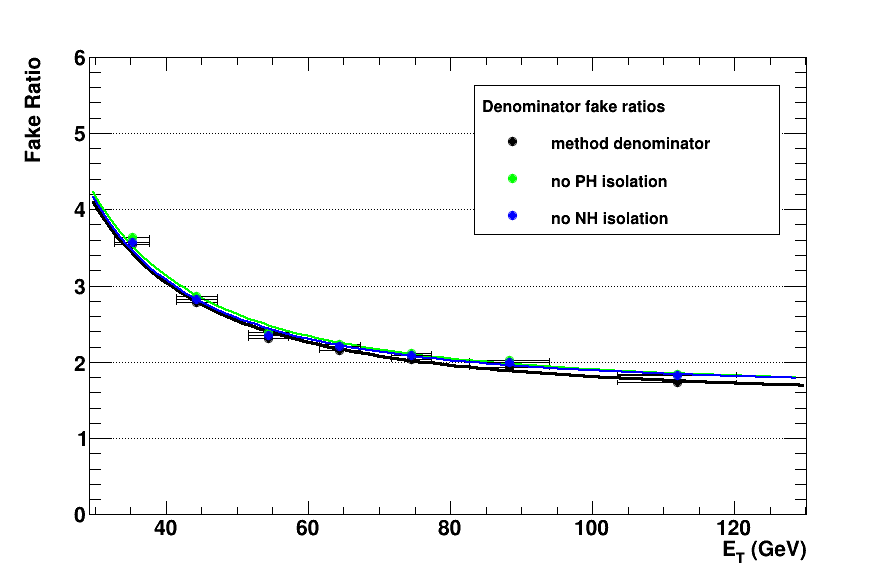
\includegraphics[width=0.45\textwidth]{qcdPlots/qcd_fitResult_deno}
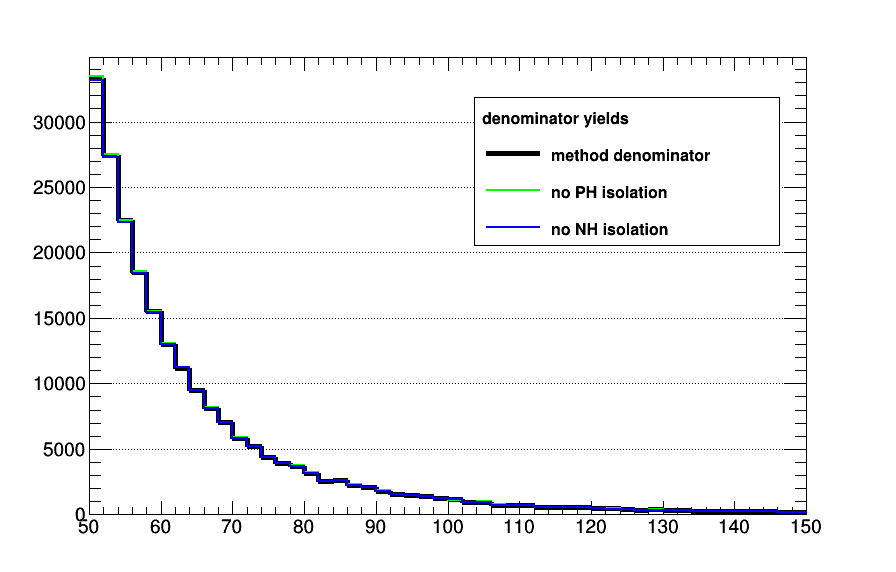
\includegraphics[width=0.45\textwidth]{qcdPlots/qcd_denoYields}
\caption{Corrected fake ratio as a function of photon \et for different denominator definitions and the final corresponding yields in our analysis data.}
\label{fig:fit_DENOMsys}
\end{figure}

\begin{itemize}
\item \met dependence
\end{itemize}

Regarding \textbf{missing transverse energy} dependence we have examined the dependence of the final fake ratio on \met.
We have calculated the fake ratio again as a function of both \met and $\ET^{\gamma}$. Fig. \ref{fig:fit_METsyspartial} shows the corresponding fake ratios as a function of $\ET^{\gamma}$ for various \met regions.  An additional test was made including our signal region, shown in figure \ref{fig:fit_METallsys}.

\begin{figure}[!h]
\begin{center}
{\label{fig:fit_METsyspartial}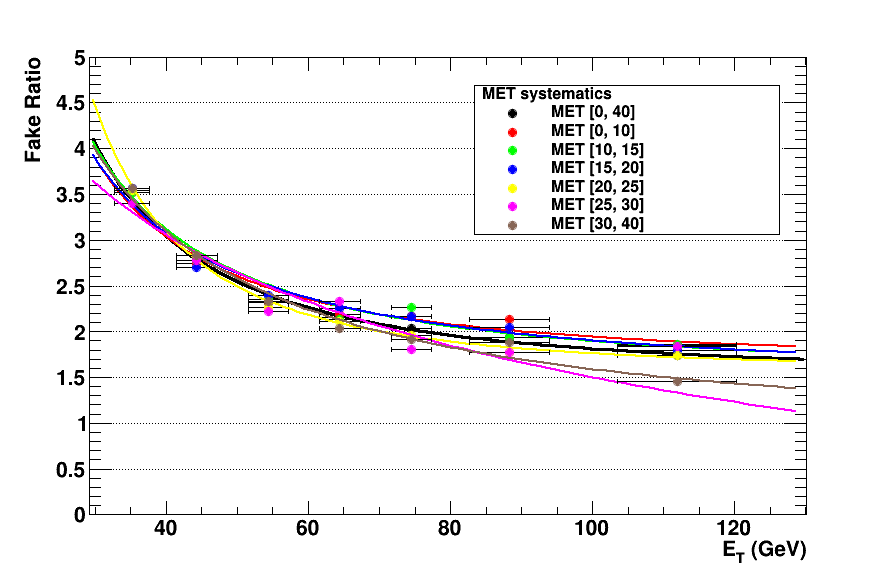
\includegraphics[width=0.45\textwidth]{qcdPlots/qcd_fitResult_MET40}}
{\label{fig:fit_METallsys}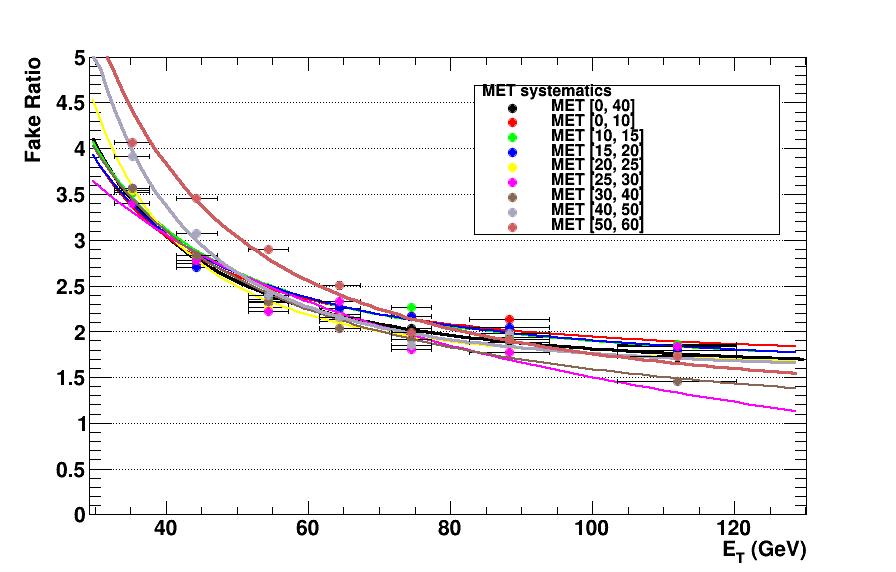
\includegraphics[width=0.45\textwidth]{qcdPlots/qcd_fitResult_allMET}}
\caption{Corrected fake ratio as a function of photon \et for different \met regions.}
\label{fig:fit_METsys}
\end{center}
\end{figure}

\begin{itemize}
\item Sideband selection for the fake templates
\end{itemize}

Finally to compute the systematics coming from the \textbf{sideband selection} for our fake templates we have recomputed the fake ratio changing the sideband selection, closer to the "real photon" region and closer to the "fake photon" region. Fig. \ref{fig:fit_SIDEBANDsys} shows the corresponding fake ratios.

\begin{figure}[hbtp]
\begin{center}
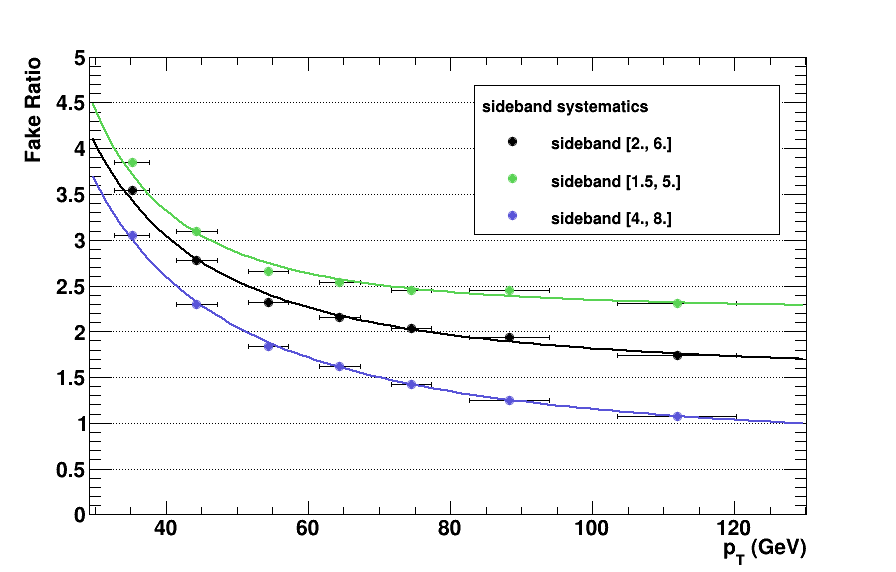
\includegraphics[width=0.7\columnwidth]{qcdPlots/qcd_fitResult_SB}
\caption{Corrected fake ratio as a function of photon \et for different sideband definitions.}
\label{fig:fit_SIDEBANDsys}
\end{center}
\end{figure}

As can be seen from above, the systematics associated with the sideband selection for our fake templates is proven to be the dominant one with ~35\%. This uncertainty is consistent with the other analysis (Exotica Diphoton and High Pt Monophoton) usign a similar approach to estimate jet faking photon background.

%%%%%%%%%%%%%%%%%%%%%%%%%%%%%%%%%%%%%%%%%%%%%%%%%%%%%%%%%%%%%%%%%%%%%%%%%%%%%%%%%%%%%%%%%%%%%%%%%%%%%%%%%%%%%%%%%%%%%%%%%%%%%%%%%%%%%%%%%%%%%%%%%%%%%%%%%%%%%%%%%%%%%%
\subsubsection{Closure test for jet $\rightarrow$ photon misidentification ratio measurement}

A closure test on the method was also performed in order to assure that our method closes well on MC.
We have performed the fake ratio method in our MC QCD samples and compared it with the fake ratio coming from MC truth information. 
The method and MC truth final fits and their ratio are presented in Fig. \ref{fig:qcd_closureTest1}.

%\begin{figure}[!h]
\begin{figure}[hbtp]
\begin{center}
%{\label{fig:qcd_closurefit}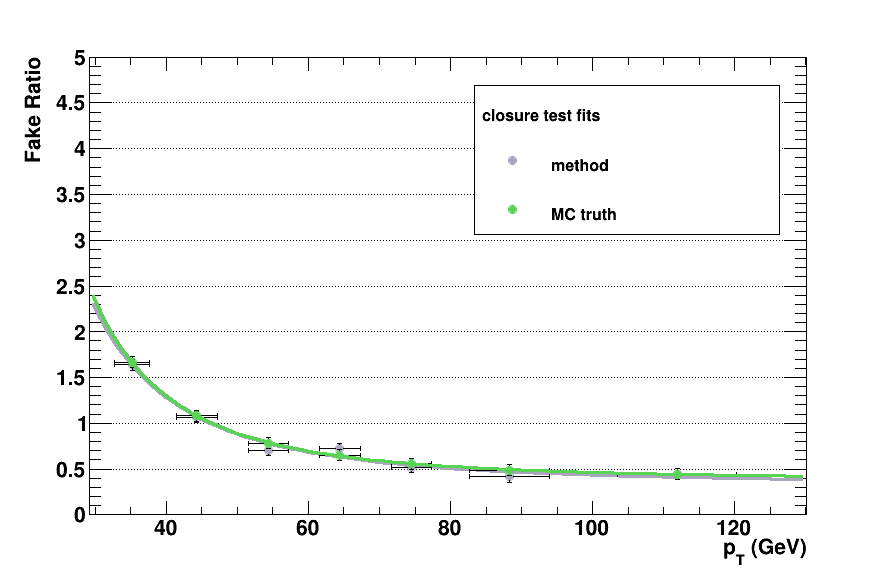
\includegraphics[width=0.45\textwidth]{qcdPlots/qcd_closureTest_fits}}
%{\label{fig:qcd_closureratio}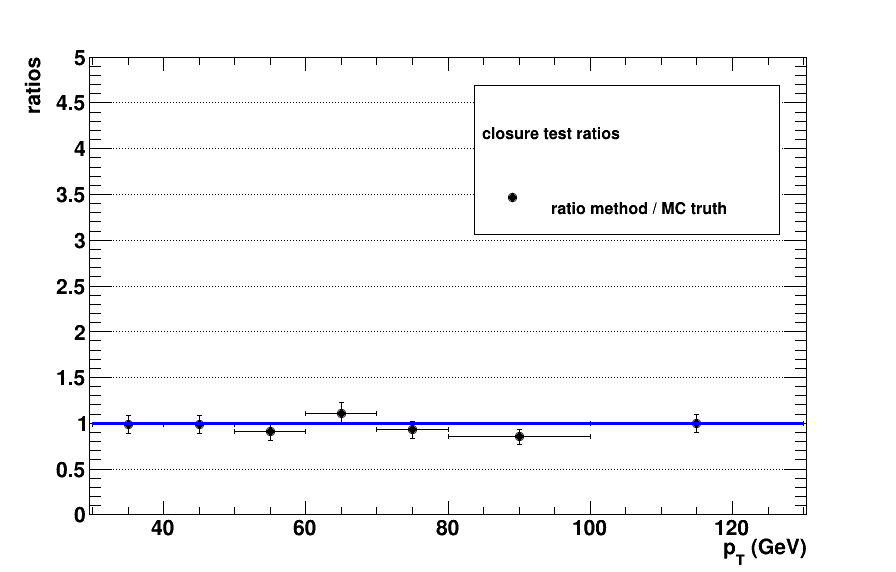
\includegraphics[width=0.45\textwidth]{qcdPlots/qcd_closureTest_ratio}}
%\caption{Closure test on the method. (a) Fake ratio method and MC truth fake ratio fits comparison and (b) their ratio, using QCD MC.}
%\label{fig:qcd_closure}
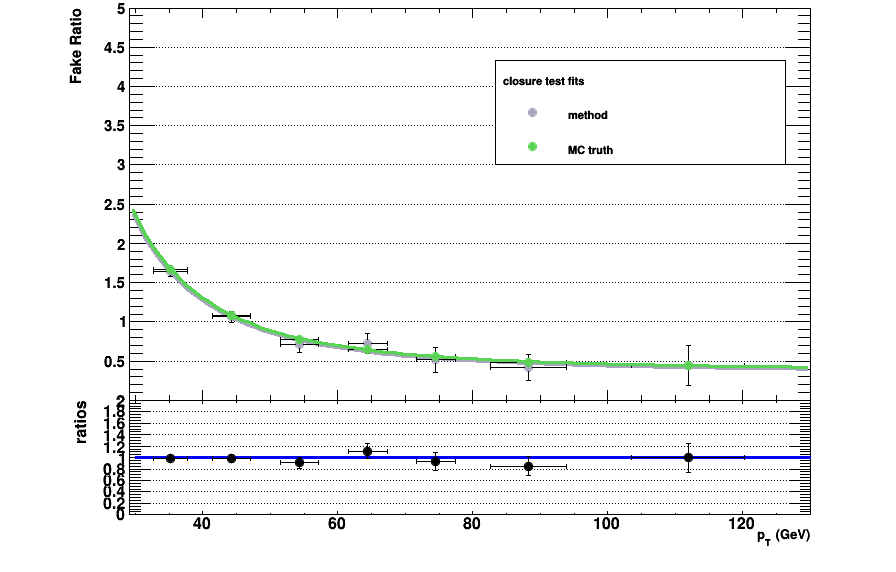
\includegraphics[width=0.7\columnwidth]{qcdPlots/qcd_closureTest1}
\caption{Closure test on the method. Fake ratio method and MC truth fake ratio fits comparison and their ratio, using QCD MC.}
\label{fig:qcd_closureTest1}
\end{center}
\end{figure}

In particular for the ratio method applyed on QCD MC we have constructed numerator, denominator and fake templates using QCD MC exactly as our data,
applying the same criteria as in our control sample. Real templates are again the ones used above, taken from $\gamma$ Jet sample.
Regarding MC truth ratio, this was constructed by using generated particle information and constructing the MC truth numerator and denominator, 
subtracting all real generated photons. The comparison of the method output to the truth fake ratio shows that our method closes very well.


%%%%%%%%%%%%%%%%%%%%%%%%%%%%%%%%%%%%%%%%%%%%%%%%%%%%%%%%%%%%%%%%%%%%%%%%%%%%%%%%%%%%%%%%%%%%%%%%%%%%%%%%%%%%%%%%%%%%%%%%%%%%%%%%%%%%%%%%%%%%%%%%%%%%%%%%%%%%%%%%%%%%%%
%%%%%%%%%%%%%%%%%%%%%%%%%%%%%%%%%%%%%%%%%%%%%%%%%%%%%%%%%%%%%%%%%%%%%%%%%%%%%%%%%%%%%%%%%%%%%%%%%%%%%%%%%%%%%%%%%%%%%%%%%%%%%%%%%%%%%%%%%%%%%%%%%%%%%%%%%%%%%%%%%%%%%%

In addition to that, a second closure test has been performed. This second test is intended to check the validity of the yields in the signal region. 
The procedure followed is described below. The general idea is to compare the QCD yield prediction of our method (fake ratio method) with the actual yield of fakes, on our candidate sample, which is obtained 
by reversing the \met cut, requirring $\met > 40 GeV$. As described above we apply the fake ratio function we have obtained, to objects passing denominator criteria 
in our candidate sample (i.e. $\met > 40 GeV$). In order to obtain the fake yield in our candidate sample, we construct 
numerator and fake templates per photon \et bin from our data, exactly as it is done in our method, apart from the $\met > 40 GeV$ cut. Real templates are again taken 
from MC, for $\met > 40 GeV$. We then again fit real and fake to numerator data and obtain the fake yield per photon \et bin, for $\sigma_{i\eta i\eta} < 0.011$. 
That means that by taking the ratio of fake yield over numerator yield for $\sigma_{i\eta i\eta} < 0.011$ we can obtain the fake fraction per photon \et bin in our 
candidate sample. We finally fit these bins and take the corresponding fake function for our candidate sample. Our candidate events are in fact numerator events with 
$\met > 40 GeV$ and $\sigma_{i\eta i\eta} < 0.011$. Applying this function on numerator events we obtain the yield of fakes in this sample. This yield is then compared
to the yield of fake ratio method. 

The fact that we are working on events with $\met > 40 GeV$, is making our samples sensitive to beam halo. In particular our templates are contaminated by beam halo events
as $\sigma_{i\eta i\eta}$ is left free in order to constuct the templates and perform the fitting. The $\sigma_{i\phi i\phi} > 0.001$ cut does not reject these events 
which are occuring at the area of $\sigma_{i\eta i\eta} > 0.015$. The above issue is shown in Fig. \ref{fig:template4_no_cut}.

\begin{figure}[!h]
\begin{center}
{\label{fig:template4_no_cut}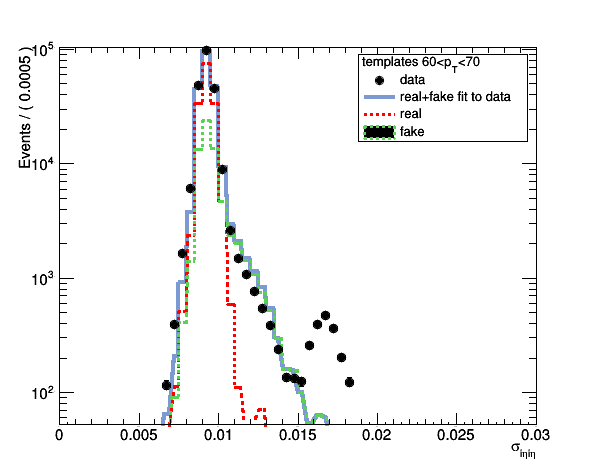
\includegraphics[width=5.5cm,height=4.3cm]{qcdPlots/template4_no_cut}}
{\label{fig:template4_sipip_cut}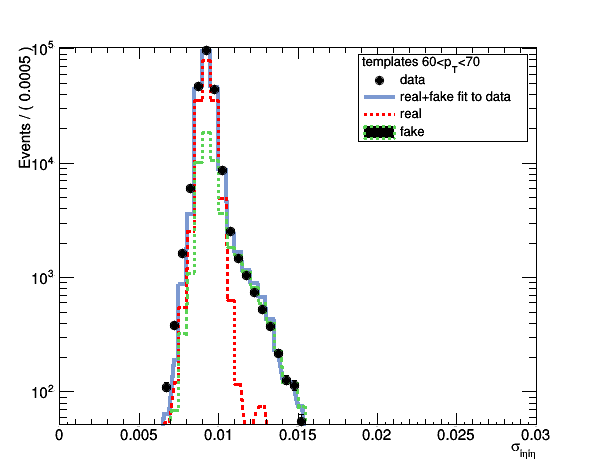
\includegraphics[width=5.5cm,height=4.3cm]{qcdPlots/template4_sipip_cut}}
{\label{fig:template4_sinin_cut}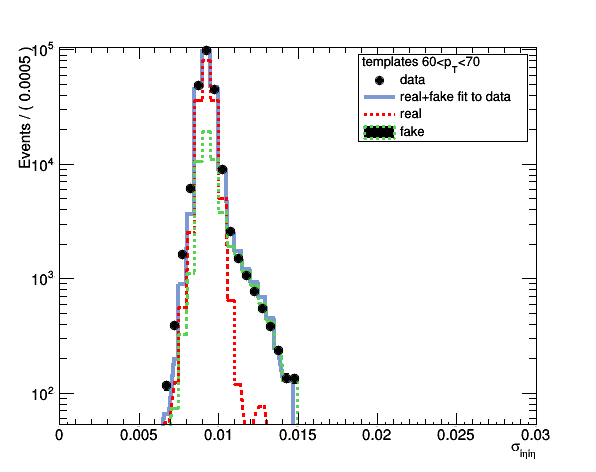
\includegraphics[width=5.5cm,height=4.3cm]{qcdPlots/template4_sinin_cut}}
\caption{$\sigma_{i\eta i\eta}$ templates for the 4th bin (a) without any harder cut, (b) with a harder $\sigma_{i\phi i\phi}$ cut, (c) with a $\sigma_{i\eta i\eta}$ cut.}
\label{fig:qcd_closure2_template4}
\end{center}
\end{figure}

The occurrence of beam halo events spoils our template fitting and as a result, the final fake yield. Fig. \ref{fig:template4_sipip_cut} shows the template fitting
for the same bin if a harder beam halo cut is applied, in particular $\sigma_{i\phi i\phi} > 0.009$. This results in rejecting mostly beam halo and obtaining a good fitting. 
However as we do not have a $\sigma_{i\phi i\phi} > 0.009$ cut in our analysis, we could find another way to reject it. In fact by observing that beam halo lives in the 
$\sigma_{i\eta i\eta} > 0.015$ area we could probably restrict our template area in the region of $0.001 < \sigma_{i\eta i\eta} > 0.015$. The corresponding template fitting 
is shown in Fig. \ref{fig:template4_sinin_cut} for the fourth bin. Of course we should prove that these two methods give the same results.

\begin{figure}[hbtp]
\begin{center}
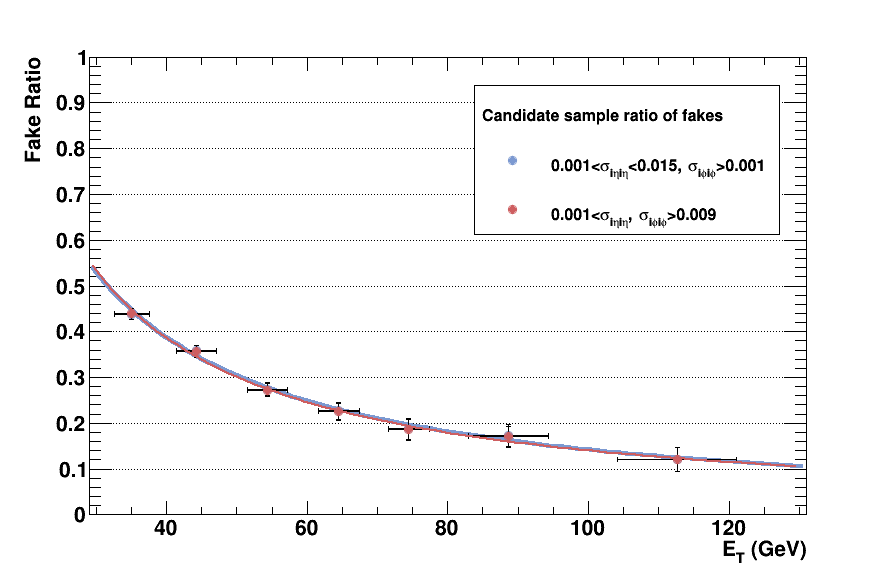
\includegraphics[width=0.6\columnwidth]{qcdPlots/fakeRatioFits_Sipip_Sinin}
\caption{Comparison of the fake ratio functions on candidate sample by putting a harder $\sigma_{i\phi i\phi}$ or a harder $\sigma_{i\eta i\eta}$ cut in our templates.}
\label{fig:fakeRatioFits_Sipip_Sinin}
\end{center}
\end{figure}

Fig. \ref{fig:fakeRatioFits_Sipip_Sinin} shows that the results on the final fit are almost identical. The final function of fakes to be applied on numerator data is 
shown in Fig.~\ref{fig:fitResult_closure2}.
Finally we apply this fake ratio function to numerator and compare it to the method prediction. Fig.~\ref{fig:closeYields} shows the comparison of the yields of these  two methods and the corresponding ratio obtained by dividing the fake ratio yield to the yield of our method.

\begin{figure}[hbtp]
\begin{center}
{\label{fig:fitResult_closure2}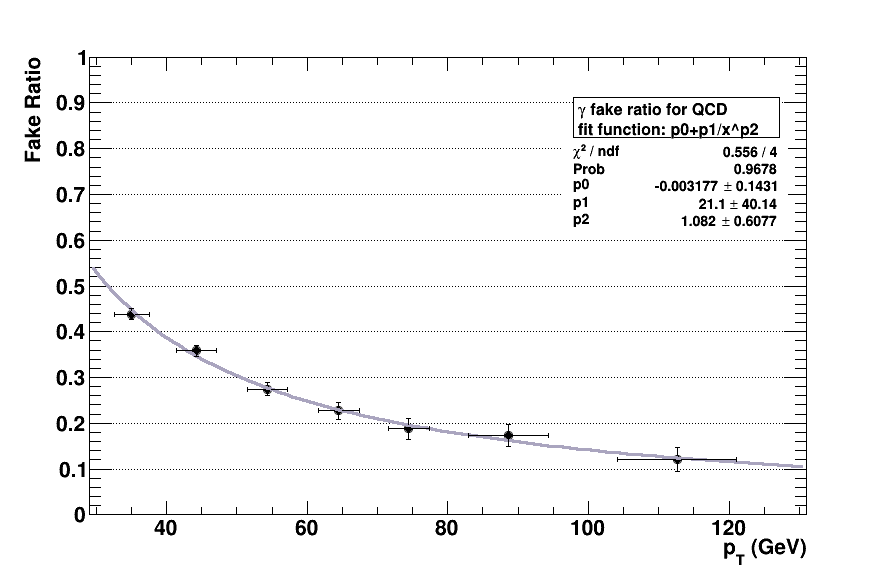
\includegraphics[width=0.45\textwidth]{qcdPlots/fitResult_closure2}}
{\label{fig:closeYields}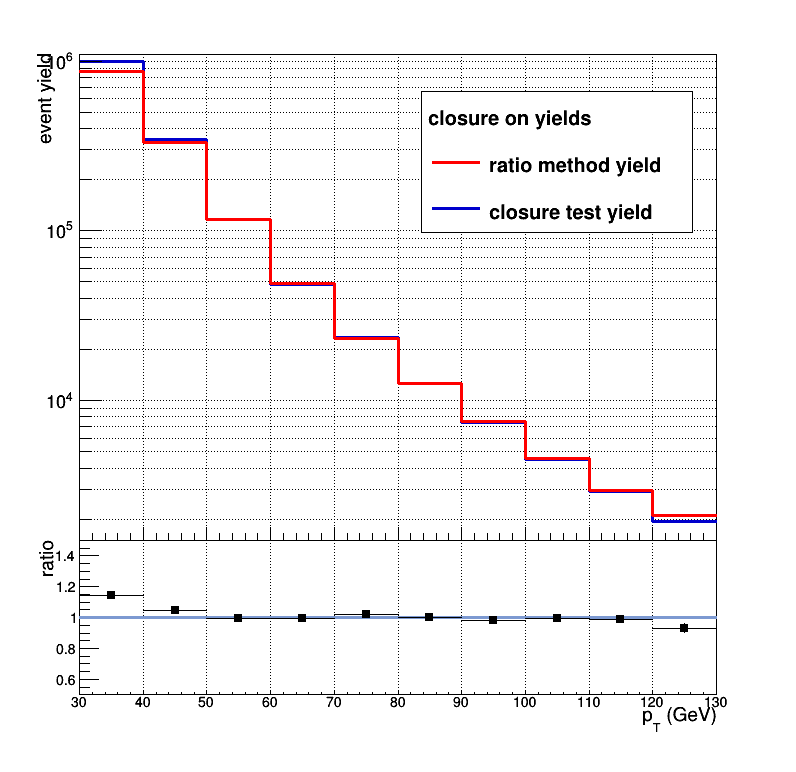
\includegraphics[width=0.45\textwidth]{qcdPlots/closeYields}}
\caption{Fit result of ratio of fakes in numerator data on the left, and comparision of the yields with on the right.}
\label{fig:fitResult_closure2_all}
\end{center}
\end{figure}

Through investigating various closure test methods, we have conlcuded that our estimations on the jet faking a photon background is reliable within the above mentioned systematics.

%%%%%%%%%%%%%%%%%%%%%%%%%%%%%%%%%%%%%%%%%%%%%%%%%%%%%%%%%%%%%%%%%%%%%%%%%%%%%%%%%%%%%%%%%%%%%%%%%%%%%%%%%%%%%%%%%%%%%%%%%%%%%%%%%%%%%%%%%%%%%%%%%%%%%%%%%%%%%%%%%%%%%%
%%%%%%%%%%%%%%%%%%%%%%%%%%%%%%%%%%%%%%%%%%%%%%%%%%%%%%%%%%%%%%%%%%%%%%%%%%%%%%%%%%%%%%%%%%%%%%%%%%%%%%%%%%%%%%%%%%%%%%%%%%%%%%%%%%%%%%%%%%%%%%%%%%%%%%%%%%%%%%%%%%%%%%
